\documentclass[xcolor=dvipsnames,10pt]{beamer}
\usepackage{amsmath}
\usepackage{amssymb}
\usepackage{graphicx}
\usepackage{graphics}
%\usepackage{epstopdf}
%\usepackage{epsfig}

%%%%%% FONTS %%%%%%%
%\usepackage[T1]{fontenc}
%\usepackage{helvet}
%\usepackage{charter}
\usepackage{fontspec} % xelatex
\usepackage{unicode-math}
\usepackage{lualatex-math}
%\usepackage{mathptmx} %times font for math
\setmainfont{TexGyreTermes}
\setmathfont[math-style=upright]{TeXGyreTermesMath}
%\usepackage[uprightGreek]{newtxmath}
\usepackage{FiraSans}
\usefonttheme[onlymath]{serif}
%%%%%%%%%%%%%%%%%%%





\usepackage{tikz}
\usetikzlibrary{shapes,snakes}
\usetikzlibrary{arrows}

% \usepackage{url}
\usepackage[normalem]{ulem}
\newcommand{\one}{\ensuremath{\bar{\mathsf{1}}}}
\newcommand{\zero}{\ensuremath{\bar{\mathsf{0}}}}
\newcommand{\prob}{\ensuremath{\mathbf{P}}}
\newcommand{\expec}{\ensuremath{\mathbf{E}}}  
\newcommand{\ind}{\ensuremath{\mathbf{I}}}
\newcommand{\reals}{\ensuremath{\mathbb{R}}}
\newcommand{\defeq}{\ensuremath{\triangleq}}
\newcommand{\argmax}{\ensuremath{\mathop{\text{argmax}}\limits}}








\newtheorem{cor}{Corollary}
\newtheorem{remark}{Remark}
\newtheorem{assumption}{Assumption}


\newcommand{\BR}{\mathbf{BR}} % Best response
\title{{\textbf{\textcolor{GreenYellow}{Best Response Map}}}}
\author{\textcolor{MidnightBlue}{\bf Prof. Krishnamurthy Iyer}\\
{\small ORIE 4350, Introduction to Game Theory}}
%Joint work with\\  Ramesh Johari, Stanford University, and\\ Mukund Sundararajan, Google Inc.}
\date{\today\\ \copyright All rights reserved}
%\\ \texttt{kriyer@stanford.edu}}



%% Following is for the outline slide to show up during 
%% section changes.
\AtBeginSection[] %Change to Section
{
  \begin{frame}<beamer>
    \frametitle{Outline}
    \tableofcontents[currentsection,currentsubsection]
  \end{frame}
}



%% Following is for page number format
%% values : arabic, alph, roman
%\pagenumbering{arabic}

%% Following is to show page numbers on the slide
%% values : page number, frame number
% \setbeamertemplate{footline}[frame number]
%\setbeamertemplate{footline}[text line]{%
%  \parbox{\linewidth}{\vspace*{-10pt}Krishnamurthy Iyer, \textcopyright 2015 }}

%% Following removes the navigation bar from the slide
\beamertemplatenavigationsymbolsempty

%% Theme 
\usetheme{Rochester}
\usecolortheme[RGB={55,60,60}]{structure} 
%\useinnertheme[shadow=true]{rounded}

\setbeamerfont{frametitle}{series=\bfseries,parent=structure}
\setbeamercolor{frametitle}{fg=GreenYellow}
\begin{document}

\begin{frame}
\titlepage
\end{frame}

% \begin{frame}
%   \frametitle{Outline}
%   \tableofcontents
%   % You might wish to add the option [pausesections]
% \end{frame}


\begin{frame}{Best response map}
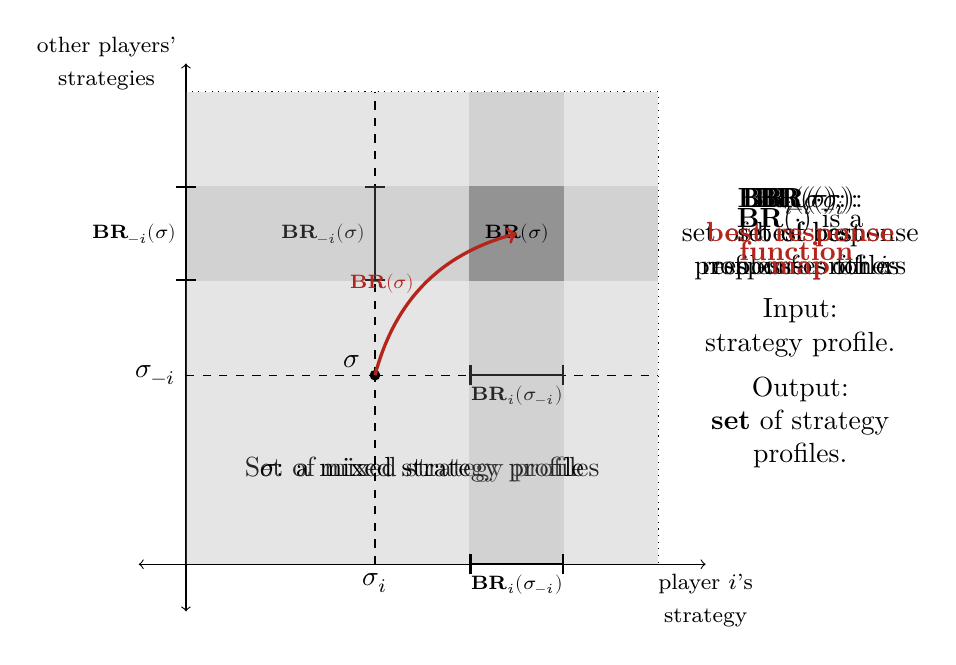
\begin{tikzpicture}[scale=1.2,domain=0:6]
    \coordinate (A) at (2,2);
    \coordinate (B) at (2,0);
    \coordinate (C) at (0,2);
    \coordinate (D) at (3,0);
    \coordinate (E) at (4,0);
    \coordinate (F) at (4,5);
    \coordinate (G) at (3,5);
    \coordinate (H) at (3,2);
    \coordinate (HH) at (5,2);
    \coordinate (I) at (4,2);
    \coordinate (J) at (0,3);
    \coordinate (K) at (0,4);
    \coordinate (L) at (5,4);
    \coordinate (M) at (5,3);
    \coordinate (N) at (2,3);
    \coordinate (NN) at (2,5);
    \coordinate (O) at (2,4);
    \coordinate (P) at (3,3);
    \coordinate (Q) at (4,3);
    \coordinate (R) at (4,4);
    \coordinate (S) at (3,4);
    \coordinate (T) at (3.5,3.5);
    \coordinate (U) at (2.5,1);
    \coordinate (V) at (6.5,3.5);
    \coordinate (W) at (6.5,2.5);
    \coordinate (X) at (6.5,1.5);


    \draw[dotted] (0,0) rectangle (5,5);
%\draw[dotted,color=gray] (-0.1,-0.1) grid (5,5);
    \draw[<->] (-0.5,0) -- (5.5,0) node[below, align=center] {\footnotesize player $i$'s\\ \footnotesize strategy};
    \draw[<->] (0,-0.5) -- (0,5.3) node[left, align=center] {\footnotesize other players' \\ \footnotesize strategies};

    \onslide<2>{
      \node at (U) {Set of mixed strategy profiles};
      \fill[gray!80, nearly transparent] (0,0) rectangle(5,5);
    }
    


    \onslide<3->{\draw[fill=black] (A) circle(0.05);}
    \onslide<3,4,5,6,7,20->{\node[above=5,left=2] at (A) {$\sigma$};}
    \onslide<4>{
      \node at (U) {$\sigma$: a mixed strategy profile};
    }
    


    \onslide<6-19>{
      \draw[dashed] (B) -- (A);
      \node[below] at (B) {$\sigma_i$};
    }
    \onslide<7-19>{
      \draw[dashed] (C) -- (A);
      \node[left] at (C) {$\sigma_{-i}$};
    }
    \onslide<9-11>{
     \draw[dashed] (A) -- (HH);
}

    \onslide<10-11>{
      
      %\draw[|-|,thick] (D) -- node[midway,below]{\scriptsize  $\BR_i(\sigma_{-i})$} (E);
      \draw[|-|,thick] (H) -- node[midway,below]{\scriptsize  $\BR_i(\sigma_{-i})$} (I);
    }


    \onslide<10>{
      \node[align=center] at (V) {$\BR_i(\sigma_{-i})$:\\ set of best\\ responses for $i$};
    }


    \onslide<11-19>{
      \fill[gray!80,nearly transparent] (D)--(E)--(F)--(G) -- cycle;
      
    }
      
    \onslide<12-19>{
      \draw[|-|, thick] (D) -- node[midway,below]{\scriptsize $\BR_i(\sigma_{-i})$} (E);      
    }


    \onslide<13-16>{
      \draw[dashed] (A) -- (NN);
    }


    \onslide<14-16>{
      \draw[|-|,thick] (N) -- node[midway,left]{\scriptsize  $\BR_{-i}(\sigma)$} (O);

    }

    \onslide<15>{
      \node[align=center] at (V) {$\BR_{-i}(\sigma)$:\\ set of best response\\ profiles for others};
    }

    \onslide<16-19>{
      \fill[gray!80,nearly transparent] (J)--(K)--(L)--(M) -- cycle;
    }
    
    \onslide<17-19>{
      \draw[|-|, thick] (J) -- node[midway,left]{\scriptsize $\BR_{-i}(\sigma)$} (K);      
    }


    \onslide<18->{
      \fill[gray!200,nearly transparent] (P)--(Q)--(R)--(S) -- cycle;      
    }

    \onslide<19,20>{
      \node at (T) {\scriptsize $\BR(\sigma)$};
    }

    \onslide<20>{
      \node[align=center] at (V) {$\BR(\sigma)$:\\ set of best\\ response profiles};
     }

    
    % \onslide<13-15>{
    %   \fill[gray!80,nearly transparent] (J)--(K)--(L)--(M) -- cycle;
    %   \draw[|-|,thick] (N) -- node[midway,left]{\scriptsize  $\BR_{-i}(\sigma)$} (O);
    %   \draw[dashed] (A) -- (NN);
    % }


    % \onslide<10>{
    %   \node[align=center] at (V) {$\BR_{-i}(\sigma)$:\\ set of best response\\ profiles for others};
    % }

    % \onslide<11-15>{
    %   \fill[gray!200,nearly transparent] (P)--(Q)--(R)--(S) -- cycle;
    % }
    % \onslide<12-13>{
    %   \node at (T) {\scriptsize $\BR(\sigma)$};
    % }
    % \onslide<13>{
    %   \node[align=center] at (V) {$\BR(\sigma)$:\\ set of best\\ response profiles};
    % }


    \onslide<21->{
      \path[->,very thick,color=BrickRed] (A) edge[bend left] node[left] {\scriptsize $\BR(\sigma)$} (T);
    }
    \onslide<21>{
      \node[align=center] at (V) {$\BR(\cdot)$:\\ \textcolor{BrickRed}{\textbf{best response}}\\ \textcolor{BrickRed}{\textbf{map}}};    
    }

    \onslide<22>{
      \node[align=center] at (V) {$\BR(\cdot)$ is a\\ \textbf{\textcolor{BrickRed}{function}}.};    
      \node[align=center] at (W) {Input:\\ strategy profile.}; 
      \node[align=center] at (X) {Output:\\ \textbf{set} of strategy\\ profiles.};    
    }



\end{tikzpicture}
\end{frame}


\begin{frame}{Best response map}
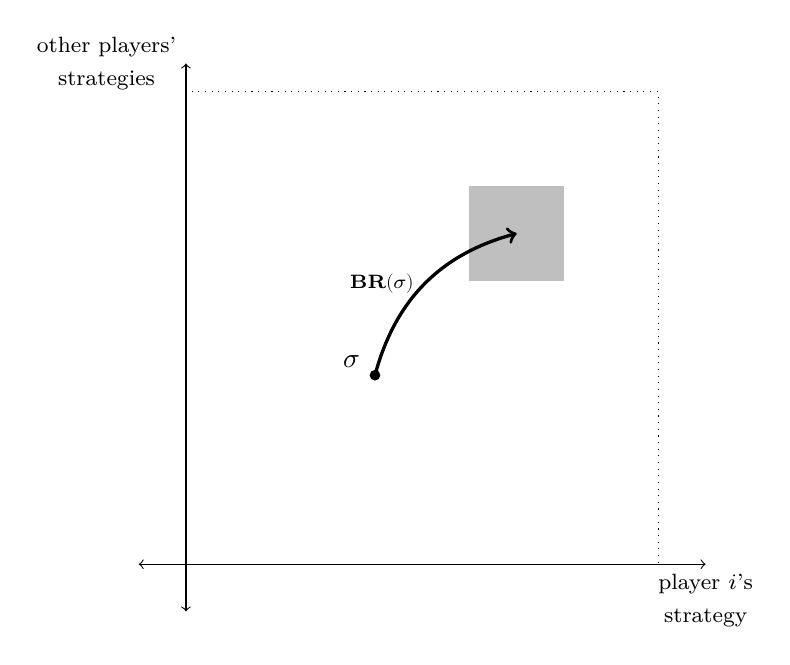
\begin{tikzpicture}[scale=1.2,domain=0:6]
    \coordinate (A) at (2,2);
    \coordinate (P) at (3,3);
    \coordinate (Q) at (4,3);
    \coordinate (R) at (4,4);
    \coordinate (S) at (3,4);
    \coordinate (T) at (3.5,3.5);
    \draw[dotted] (0,0) rectangle (5,5);
    % \draw[dotted,color=gray] (-0.1,-0.1) grid (5,5);
    \draw[<->] (-0.5,0) -- (5.5,0) node[below, align=center] {\footnotesize player $i$'s\\ \footnotesize strategy};
    \draw[<->] (0,-0.5) -- (0,5.3) node[left, align=center] {\footnotesize other players' \\ \footnotesize strategies};
    \draw[fill=black] (A) circle(0.05);
    \node[above=5,left=2] at (A) {$\sigma$};
    \fill[gray!200,nearly transparent] (P)--(Q)--(R)--(S) -- cycle;
    \path[->,very thick] (A) edge[bend left] node[left] {\scriptsize $\BR(\sigma)$} (T);
\end{tikzpicture}
\end{frame}


\begin{frame}{Best response map}
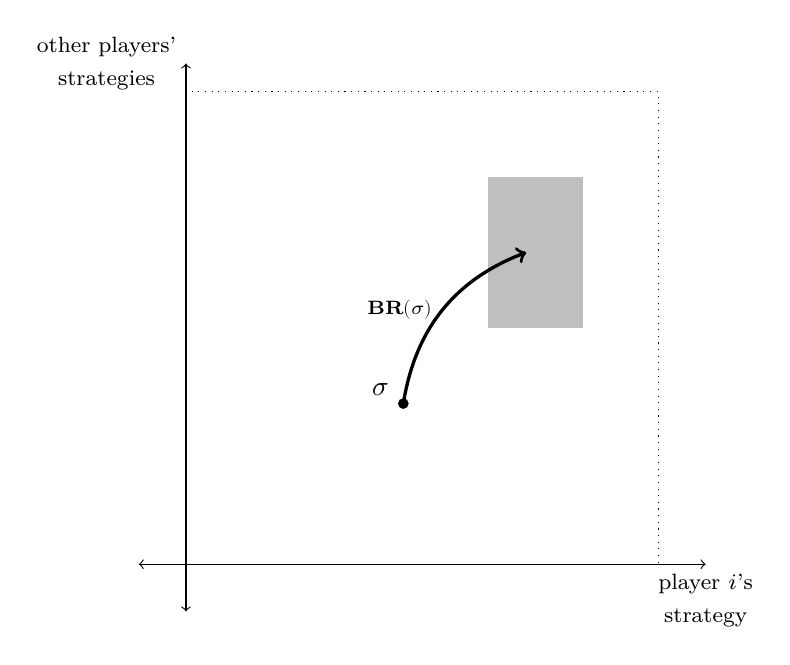
\begin{tikzpicture}[scale=1.2,domain=0:6]
    \coordinate (A) at (2.3,1.7);
    \coordinate (P) at (3.2,2.5);
    \coordinate (Q) at (4.2,2.5);
    \coordinate (R) at (4.2,4.1);
    \coordinate (S) at (3.2,4.1);
    \coordinate (T) at (3.6,3.3);
    \draw[dotted] (0,0) rectangle (5,5);
    % \draw[dotted,color=gray] (-0.1,-0.1) grid (5,5);
    \draw[<->] (-0.5,0) -- (5.5,0) node[below, align=center] {\footnotesize player $i$'s\\ \footnotesize strategy};
    \draw[<->] (0,-0.5) -- (0,5.3) node[left, align=center] {\footnotesize other players' \\ \footnotesize strategies};
    \draw[fill=black] (A) circle(0.05);
    \node[above=5,left=2] at (A) {$\sigma$};
    \fill[gray!200,nearly transparent] (P)--(Q)--(R)--(S) -- cycle;
    \path[->,very thick] (A) edge[bend left] node[left] {\scriptsize $\BR(\sigma)$} (T);
\end{tikzpicture}
\end{frame}

\begin{frame}{Best response map}
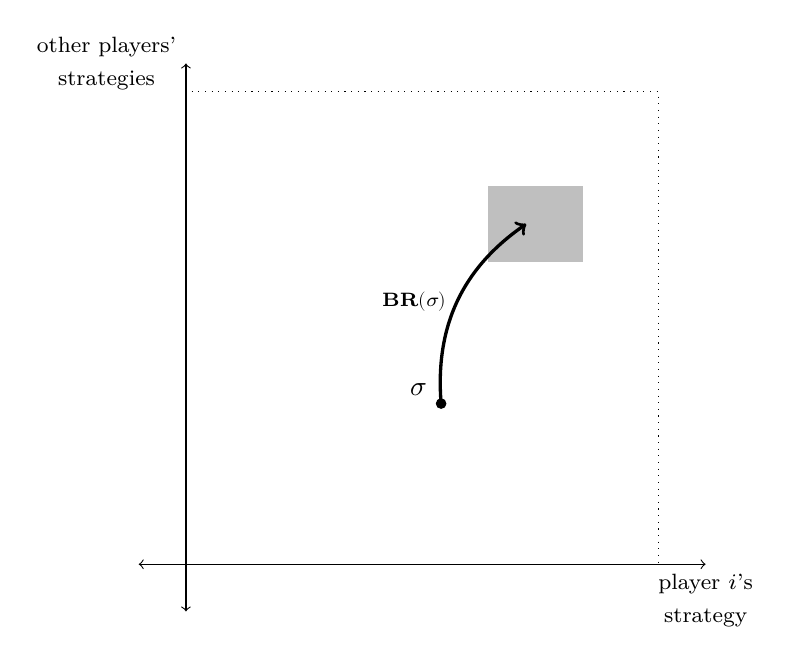
\begin{tikzpicture}[scale=1.2,domain=0:6]
    \coordinate (A) at (2.7,1.7);
    \coordinate (P) at (3.2,3.2);
    \coordinate (Q) at (4.2,3.2);
    \coordinate (R) at (4.2,4);
    \coordinate (S) at (3.2,4);
    \coordinate (T) at (3.6,3.6);
    \draw[dotted] (0,0) rectangle (5,5);
    %\draw[dotted,color=gray] (-0.1,-0.1) grid (5,5);
    \draw[<->] (-0.5,0) -- (5.5,0) node[below, align=center] {\footnotesize player $i$'s\\ \footnotesize strategy};
    \draw[<->] (0,-0.5) -- (0,5.3) node[left, align=center] {\footnotesize other players' \\ \footnotesize strategies};
    \draw[fill=black] (A) circle(0.05);
    \node[above=5,left=2] at (A) {$\sigma$};
    \fill[gray!200,nearly transparent] (P)--(Q)--(R)--(S) -- cycle;
    \path[->,very thick] (A) edge[bend left] node[left] {\scriptsize $\BR(\sigma)$} (T);
\end{tikzpicture}
\end{frame}

\begin{frame}{Best response map}
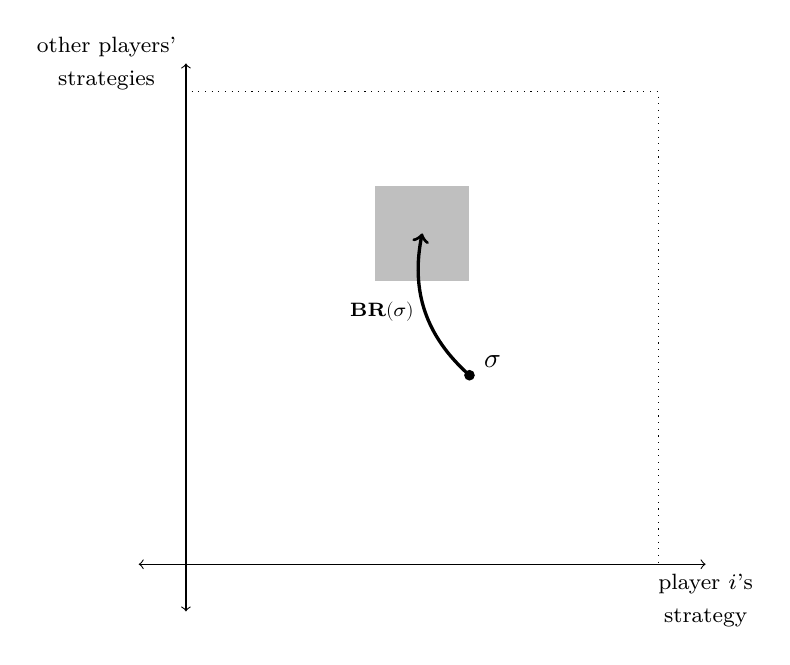
\begin{tikzpicture}[scale=1.2,domain=0:6]
    \coordinate (A) at (3,2);
    \coordinate (P) at (2,3);
    \coordinate (Q) at (3,3);
    \coordinate (R) at (3,4);
    \coordinate (S) at (2,4);
    \coordinate (T) at (2.5,3.5);
    \draw[dotted] (0,0) rectangle (5,5);
    %\draw[dotted,color=gray] (-0.1,-0.1) grid (5,5);
    \draw[<->] (-0.5,0) -- (5.5,0) node[below, align=center] {\footnotesize player $i$'s\\ \footnotesize strategy};
    \draw[<->] (0,-0.5) -- (0,5.3) node[left, align=center] {\footnotesize other players' \\ \footnotesize strategies};
    \draw[fill=black] (A) circle(0.05);
    \node[above=5,right=2] at (A) {$\sigma$};
    \fill[gray!200,nearly transparent] (P)--(Q)--(R)--(S) -- cycle;
    \path[->,very thick] (A) edge[bend left] node[left] {\scriptsize $\BR(\sigma)$} (T);
\end{tikzpicture}
\end{frame}



\begin{frame}{Best response map}
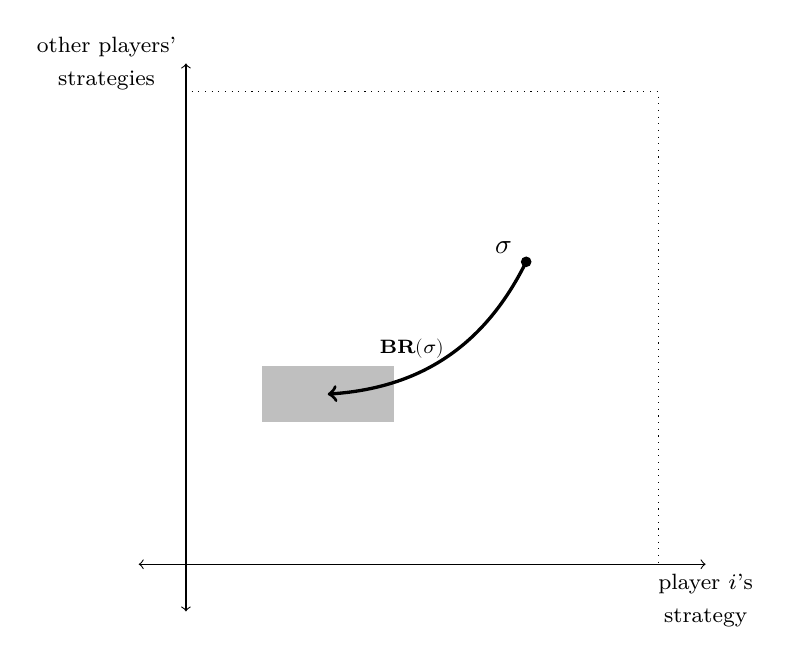
\begin{tikzpicture}[scale=1.2,domain=0:6]
    \coordinate (A) at (3.6,3.2);
    \coordinate (P) at (0.8,1.5);
    \coordinate (Q) at (2.2,1.5);
    \coordinate (R) at (2.2,2.1);
    \coordinate (S) at (0.8,2.1);
    \coordinate (T) at (1.5,1.8);
    \draw[dotted] (0,0) rectangle (5,5);
    %\draw[dotted,color=gray] (-0.1,-0.1) grid (5,5);
    \draw[<->] (-0.5,0) -- (5.5,0) node[below, align=center] {\footnotesize player $i$'s\\ \footnotesize strategy};
    \draw[<->] (0,-0.5) -- (0,5.3) node[left, align=center] {\footnotesize other players' \\ \footnotesize strategies};
    \draw[fill=black] (A) circle(0.05);
    \node[above=5,left=2] at (A) {$\sigma$};
    \fill[gray!200,nearly transparent] (P)--(Q)--(R)--(S) -- cycle;
    \path[->,very thick] (A) edge[bend left] node[above=3,left=-3] {\scriptsize $\BR(\sigma)$} (T);
\end{tikzpicture}
\end{frame}


\begin{frame}{Best response map}
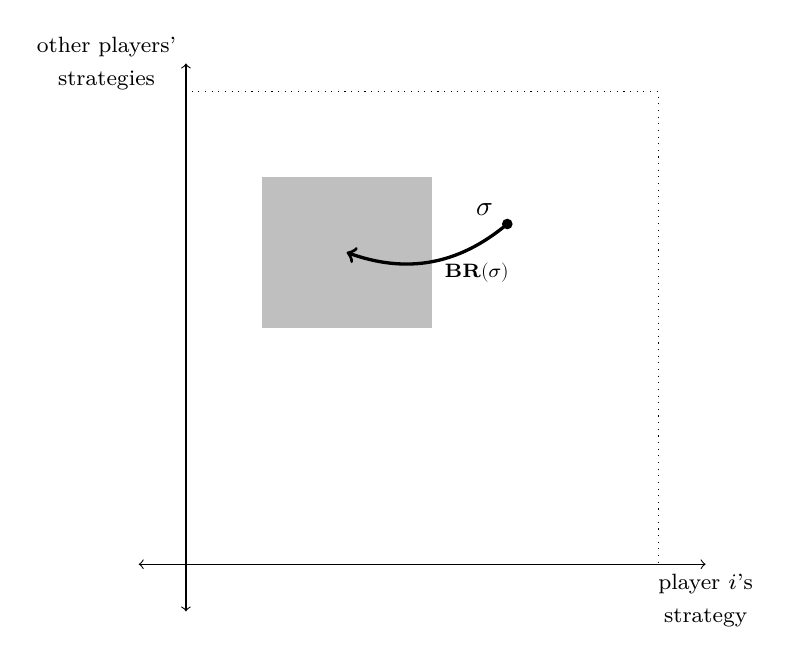
\begin{tikzpicture}[scale=1.2,domain=0:6]
    \coordinate (A) at (3.4,3.6);
    \coordinate (P) at (0.8,2.5);
    \coordinate (Q) at (2.6,2.5);
    \coordinate (R) at (2.6,4.1);
    \coordinate (S) at (0.8,4.1);
    \coordinate (T) at (1.7,3.3);
    \draw[dotted] (0,0) rectangle (5,5); 
   %\draw[dotted,color=gray] (-0.1,-0.1) grid (5,5);
    \draw[<->] (-0.5,0) -- (5.5,0) node[below, align=center] {\footnotesize player $i$'s\\ \footnotesize strategy};
    \draw[<->] (0,-0.5) -- (0,5.3) node[left, align=center] {\footnotesize other players' \\ \footnotesize strategies};
    \draw[fill=black] (A) circle(0.05);
    \node[above=5,left=2] at (A) {$\sigma$};
    \fill[gray!200,nearly transparent] (P)--(Q)--(R)--(S) -- cycle;
    \path[->,very thick] (A) edge[bend left] node[below=4,right=1] {\scriptsize $\BR(\sigma)$} (T);
\end{tikzpicture}
\end{frame}

\begin{frame}{Best response map}
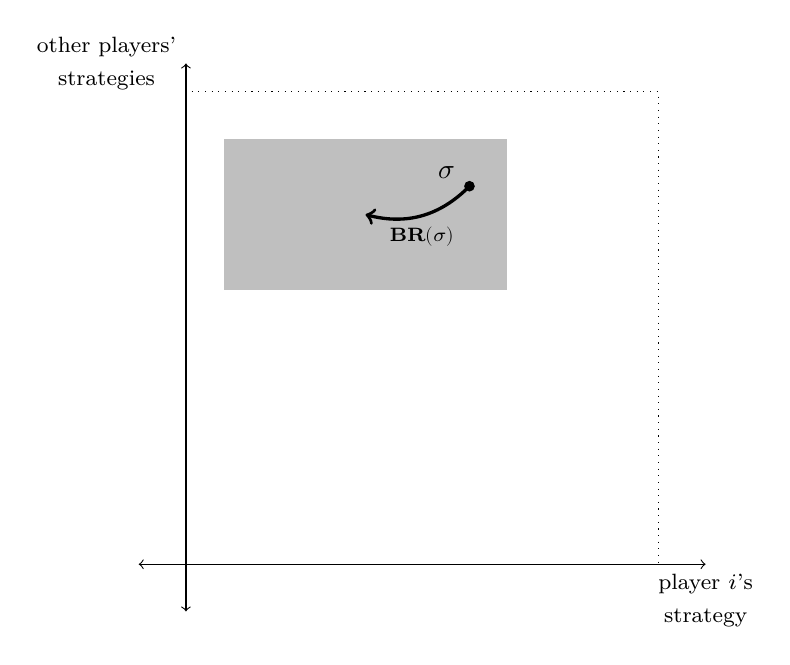
\begin{tikzpicture}[scale=1.2,domain=0:6]
    \coordinate (A) at (3.0,4.0);
    \coordinate (B) at (3.0,0);
    \coordinate (C) at (0,4.0);
    \coordinate (D) at (0.4,0);
    \coordinate (E) at (3.4,0);
    \coordinate (F) at (3.4,5);
    \coordinate (G) at (0.4,5);
    \coordinate (J) at (0,2.9);
    \coordinate (K) at (0,4.5);
    \coordinate (L) at (5,4.5);
    \coordinate (M) at (5,2.9);
    \coordinate (P) at (0.4,2.9);
    \coordinate (Q) at (3.4,2.9);
    \coordinate (R) at (3.4,4.5);
    \coordinate (S) at (0.4,4.5);
    \coordinate (T) at (1.9,3.7);
    \coordinate (U) at (2.5,1);
    \coordinate (V) at (6.5,3.5);
    \coordinate (W) at (6.5,2.5);
    \coordinate (X) at (6.5,1.5);
    \draw[dotted] (0,0) rectangle (5,5);
    %\draw[dotted,color=gray] (-0.1,-0.1) grid (5,5);
    \draw[<->] (-0.5,0) -- (5.5,0) node[below, align=center] {\footnotesize player $i$'s\\ \footnotesize strategy};
    \draw[<->] (0,-0.5) -- (0,5.3) node[left, align=center] {\footnotesize other players' \\ \footnotesize strategies};
    \draw[fill=black] (A) circle(0.05);
    \node[above=5,left=2] at (A) {$\sigma$};
    \fill[gray!200,nearly transparent] (P)--(Q)--(R)--(S) -- cycle;
    \path[->,very thick] (A) edge[bend left] node[below] {\scriptsize $\BR(\sigma)$} (T);
\end{tikzpicture}
\end{frame}



\begin{frame}{Best response map}

\begin{center}
\textbf{How does the best response map\\ relate to Nash equilibrium?}
\end{center}

\end{frame}


\begin{frame}{Best response map}
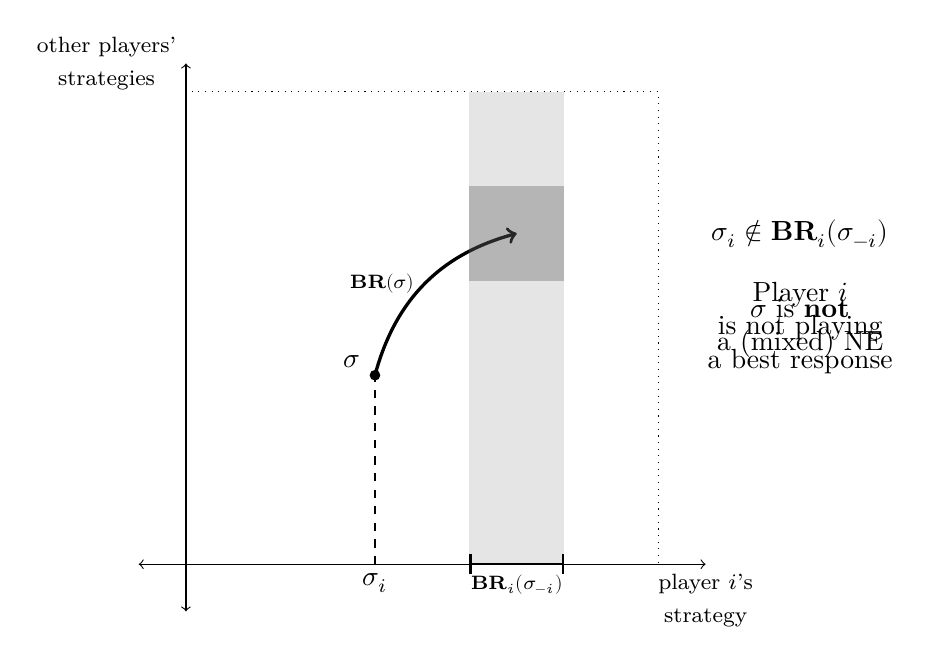
\begin{tikzpicture}[scale=1.2,domain=0:6]
    \coordinate (A) at (2,2);
    \coordinate (B) at (2,0);
    \coordinate (C) at (0,2);
    \coordinate (D) at (3,0);
    \coordinate (E) at (4,0);
    \coordinate (F) at (4,5);
    \coordinate (G) at (3,5);
    \coordinate (H) at (3,2);
    \coordinate (I) at (4,2);
    \coordinate (J) at (0,3);
    \coordinate (K) at (0,4);
    \coordinate (L) at (5,4);
    \coordinate (M) at (5,3);
    \coordinate (N) at (2,3);
    \coordinate (O) at (2,4);
    \coordinate (P) at (3,3);
    \coordinate (Q) at (4,3);
    \coordinate (R) at (4,4);
    \coordinate (S) at (3,4);
    \coordinate (T) at (3.5,3.5);
    \coordinate (U) at (2.5,1);
    \coordinate (V) at (6.5,3.5);
    \coordinate (W) at (6.5,2.5);
    \coordinate (X) at (6.5,1.5);

    \draw[dotted] (0,0) rectangle (5,5);
%\draw[dotted,color=gray] (-0.1,-0.1) grid (5,5);
    \draw[<->] (-0.5,0) -- (5.5,0) node[below, align=center] {\footnotesize player $i$'s\\ \footnotesize strategy};
    \draw[<->] (0,-0.5) -- (0,5.3) node[left, align=center] {\footnotesize other players' \\ \footnotesize strategies};
    \draw[fill=black] (A) circle(0.05);
    \node[above=5,left=2] at (A) {$\sigma$};
    \fill[gray!200,nearly transparent] (P)--(Q)--(R)--(S) -- cycle;
    \path[->,very thick] (A) edge[bend left] node[left] {\scriptsize $\BR(\sigma)$} (T);

    
    \onslide<2->{
      \draw[dashed] (B) -- (A);
      \node[below] at (B) {$\sigma_i$};
      \fill[gray!80,nearly transparent] (D)--(E)--(F)--(G) -- cycle;
      \draw[|-|, thick] (D) -- node[midway,below]{\scriptsize $\BR_i(\sigma_{-i})$} (E);
    }
    \onslide<3->{
      \node at (V) {$\sigma_i \notin \BR_i(\sigma_{-i})$};
    }
    \onslide<4>{
      \node[align=center] at (W) {Player $i$\\ is not playing\\ a best response};
    }

    \onslide<5>{
      \node[align=center] at (W) {$\sigma$ is \textbf{not}\\ a (mixed) NE};
    }
    % \onslide<6-12>{
    % }
    % \onslide<7-12>{
    %   \draw[dashed] (C) -- (A);
    %   \node[left] at (C) {$\sigma_{-i}$};
    % }
    % \onslide<9-12>{
    %   \fill[gray!80,nearly transparent] (D)--(E)--(F)--(G) -- cycle;
    %   \draw[<->] (H) -- node[midway,above]{\scriptsize  $\BR_i(\sigma_{-i})$} (I);
    %   \draw[dashed] (A) -- (H);
    % }
    %   \onslide<10-12>{
    %   \fill[gray!80,nearly transparent] (J)--(K)--(L)--(M) -- cycle;
    %   \draw[<->] (N) -- node[midway,left]{\scriptsize  $\BR_{-i}(\sigma)$} (O);
    %   \draw[dashed] (A) -- (N);
    % }
\end{tikzpicture}
\end{frame}


\begin{frame}{Best response map}
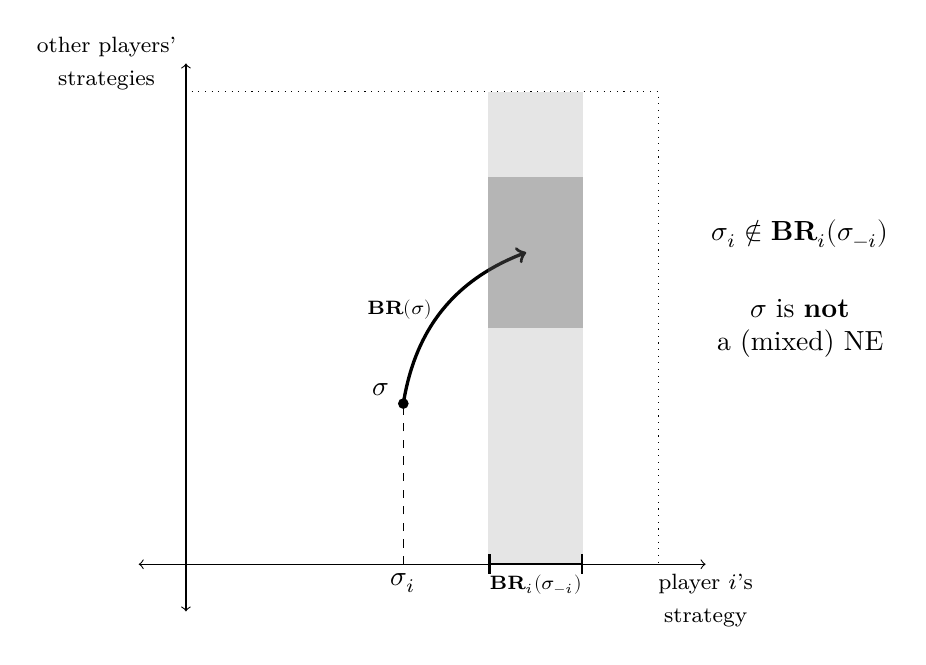
\begin{tikzpicture}[scale=1.2,domain=0:6]
    \coordinate (A) at (2.3,1.7);
    \coordinate (B) at (2.3,0);
    \coordinate (D) at (3.2,0);
    \coordinate (E) at (4.2,0);
    \coordinate (F) at (4.2,5);
    \coordinate (G) at (3.2,5);
    \coordinate (P) at (3.2,2.5);
    \coordinate (Q) at (4.2,2.5);
    \coordinate (R) at (4.2,4.1);
    \coordinate (S) at (3.2,4.1);
    \coordinate (T) at (3.6,3.3);
    \coordinate (V) at (6.5,3.5);
    \coordinate (W) at (6.5,2.5);
    \coordinate (X) at (6.5,1.5);
    \draw[dotted] (0,0) rectangle (5,5);
    %\draw[dotted,color=gray] (-0.1,-0.1) grid (5,5);
    \draw[<->] (-0.5,0) -- (5.5,0) node[below, align=center] {\footnotesize player $i$'s\\ \footnotesize strategy};
    \draw[<->] (0,-0.5) -- (0,5.3) node[left, align=center] {\footnotesize other players' \\ \footnotesize strategies};
    \draw[fill=black] (A) circle(0.05);
    \node[above=5,left=2] at (A) {$\sigma$};
    \fill[gray!200,nearly transparent] (P)--(Q)--(R)--(S) -- cycle;
    \path[->,very thick] (A) edge[bend left] node[left] {\scriptsize $\BR(\sigma)$} (T);
    \onslide<2->{
      \draw[dashed] (B) -- (A);
      \node[below] at (B) {$\sigma_i$};
      \fill[gray!80,nearly transparent] (D)--(E)--(F)--(G) -- cycle;
      \draw[|-|, thick] (D) -- node[midway,below]{\scriptsize $\BR_i(\sigma_{-i})$} (E);
    }
    \onslide<3->{
      \node at (V) {$\sigma_i \notin \BR_i(\sigma_{-i})$};
    }
    \onslide<4>{
      \node[align=center] at (W) {$\sigma$ is \textbf{not}\\ a (mixed) NE};
    }






\end{tikzpicture}
\end{frame}

\begin{frame}{Best response map}
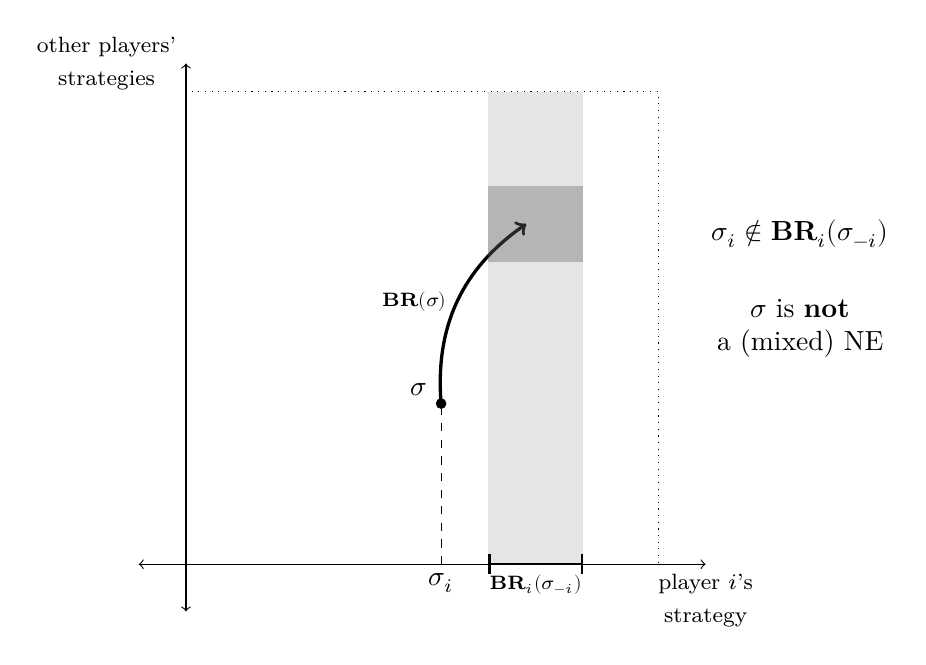
\begin{tikzpicture}[scale=1.2,domain=0:6]
    \coordinate (A) at (2.7,1.7);
    \coordinate (B) at (2.7,0);
    \coordinate (D) at (3.2,0);
    \coordinate (E) at (4.2,0);
    \coordinate (F) at (4.2,5);
    \coordinate (G) at (3.2,5);
    \coordinate (P) at (3.2,3.2);
    \coordinate (Q) at (4.2,3.2);
    \coordinate (R) at (4.2,4);
    \coordinate (S) at (3.2,4);
    \coordinate (T) at (3.6,3.6);
    \coordinate (V) at (6.5,3.5);
    \coordinate (W) at (6.5,2.5);
    \coordinate (X) at (6.5,1.5);
    \draw[dotted] (0,0) rectangle (5,5);
    %\draw[dotted,color=gray] (-0.1,-0.1) grid (5,5);
    \draw[<->] (-0.5,0) -- (5.5,0) node[below, align=center] {\footnotesize player $i$'s\\ \footnotesize strategy};
    \draw[<->] (0,-0.5) -- (0,5.3) node[left, align=center] {\footnotesize other players' \\ \footnotesize strategies};
    \draw[fill=black] (A) circle(0.05);
    \node[above=5,left=2] at (A) {$\sigma$};
    \fill[gray!200,nearly transparent] (P)--(Q)--(R)--(S) -- cycle;
    \path[->,very thick] (A) edge[bend left] node[left] {\scriptsize $\BR(\sigma)$} (T);
    \onslide<2->{
      \draw[dashed] (B) -- (A);
      \node[below] at (B) {$\sigma_i$};
      \fill[gray!80,nearly transparent] (D)--(E)--(F)--(G) -- cycle;
      \draw[|-|, thick] (D) -- node[midway,below]{\scriptsize $\BR_i(\sigma_{-i})$} (E);
    }
    \onslide<3->{
      \node at (V) {$\sigma_i \notin \BR_i(\sigma_{-i})$};
    }
    \onslide<4>{
      \node[align=center] at (W) {$\sigma$ is \textbf{not}\\ a (mixed) NE};
    }
\end{tikzpicture}
\end{frame}

\begin{frame}{Best response map}
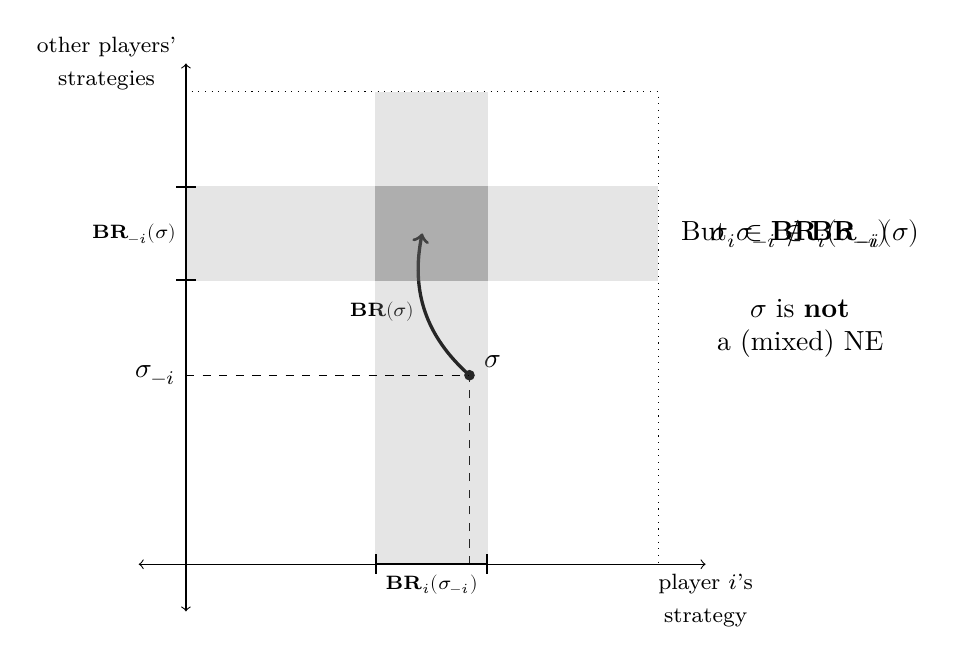
\begin{tikzpicture}[scale=1.2,domain=0:6]
    \coordinate (A) at (3,2);
    \coordinate (B) at (3,0);
    \coordinate (C) at (0,2);
    \coordinate (D) at (2,0);
    \coordinate (E) at (3.2,0);
    \coordinate (F) at (3.2,5);
    \coordinate (G) at (2,5);
    \coordinate (J) at (0,3);
    \coordinate (K) at (0,4);
    \coordinate (L) at (5,4);
    \coordinate (M) at (5,3);
    \coordinate (P) at (2,3);
    \coordinate (Q) at (3.2,3);
    \coordinate (R) at (3.2,4);
    \coordinate (S) at (2,4);
    \coordinate (T) at (2.5,3.5);
    \coordinate (V) at (6.5,3.5);
    \coordinate (W) at (6.5,2.5);
    \coordinate (X) at (6.5,1.5);
    \draw[dotted] (0,0) rectangle (5,5);
    %\draw[dotted,color=gray] (-0.1,-0.1) grid (5,5);
    \draw[<->] (-0.5,0) -- (5.5,0) node[below, align=center] {\footnotesize player $i$'s\\ \footnotesize strategy};
    \draw[<->] (0,-0.5) -- (0,5.3) node[left, align=center] {\footnotesize other players' \\ \footnotesize strategies};
    \draw[fill=black] (A) circle(0.05);
    \node[above=5,right=2] at (A) {$\sigma$};
    \fill[gray!200,nearly transparent] (P)--(Q)--(R)--(S) -- cycle;
    \path[->,very thick] (A) edge[bend left] node[left] {\scriptsize $\BR(\sigma)$} (T);
    \onslide<2>{
      \draw[dashed] (B) -- (A);
      %\node[above=8,right=-3] at (B) {$\sigma_i$};
      \fill[gray!80,nearly transparent] (D)--(E)--(F)--(G) -- cycle;
      \draw[|-|, thick] (D) -- node[midway,below]{\scriptsize $\BR_i(\sigma_{-i})$} (E);
    }

    \onslide<3->{
      \draw[dashed] (C) -- (A);
      \node[left] at (C) {$\sigma_{-i}$};
      \fill[gray!80,nearly transparent] (J)--(K)--(L)--(M) -- cycle;
      \draw[|-|, thick] (J) -- node[midway,left]{\scriptsize $\BR_{-i}(\sigma)$} (K);
    }
    \onslide<2>{
      \node at (V) {$\sigma_i \in \BR_i(\sigma_{-i})$};
    }



    \onslide<4->{
      \node at (V) {But $\sigma_{-i} \notin \BR_{-i}(\sigma)$};
    }



    \onslide<5>{
      \node[align=center] at (W) {$\sigma$ is \textbf{not}\\ a (mixed) NE};
    }
\end{tikzpicture}
\end{frame}



% \begin{frame}{Best response map}
% \begin{tikzpicture}[scale=1.2,domain=0:6]
%     \coordinate (A) at (3.6,3.2);
%     \coordinate (P) at (0.8,1.5);
%     \coordinate (Q) at (2.2,1.5);
%     \coordinate (R) at (2.2,2.1);
%     \coordinate (S) at (0.8,2.1);
%     \coordinate (T) at (1.5,1.8);
%     \coordinate (V) at (6.5,3.5);
%     \coordinate (W) at (6.5,2.5);
%     \coordinate (X) at (6.5,1.5);
%     \draw[dotted] (0,0) rectangle (5,5);
%     %\draw[dotted,color=gray] (-0.1,-0.1) grid (5,5);
%     \draw[<->] (-0.5,0) -- (5.5,0) node[below, align=center] {\footnotesize player $i$'s\\ \footnotesize strategy};
%     \draw[<->] (0,-0.5) -- (0,5.3) node[left, align=center] {\footnotesize other players' \\ \footnotesize strategies};
%     \draw[fill=black] (A) circle(0.05);
%     \node[above=5,left=2] at (A) {$\sigma$};
%     \fill[gray!200,nearly transparent] (P)--(Q)--(R)--(S) -- cycle;
%     \path[->,thick] (A) edge[bend left] node[above=3,left=-3] {\scriptsize $\BR(\sigma)$} (T);
% \end{tikzpicture}
% \end{frame}


\begin{frame}{Best response map}
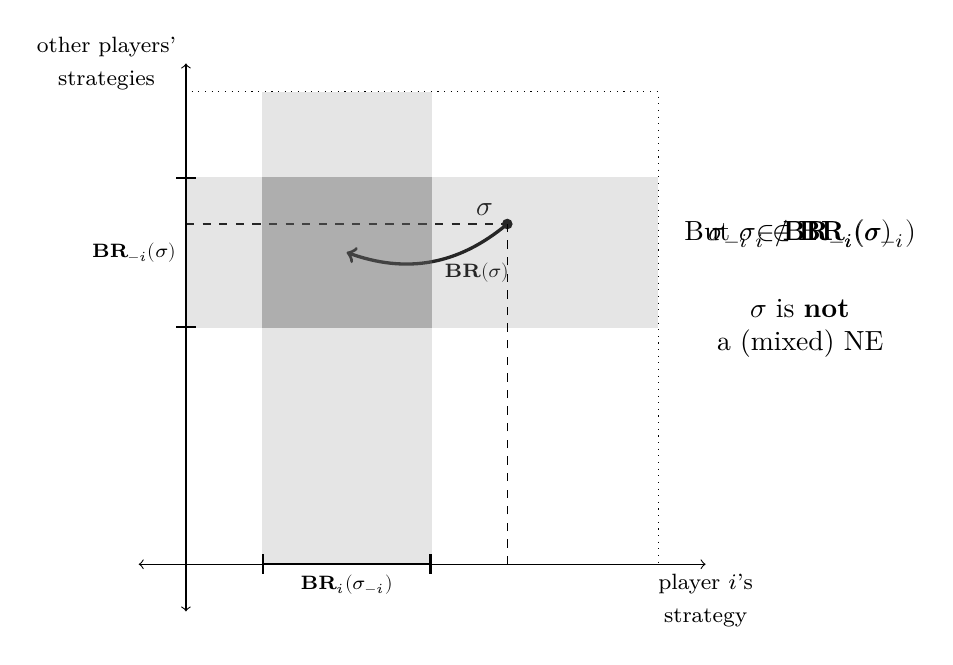
\begin{tikzpicture}[scale=1.2,domain=0:6]
    \coordinate (A) at (3.4,3.6);
    \coordinate (B) at (3.4,0);
    \coordinate (C) at (0,3.6);
    \coordinate (D) at (0.8,0);
    \coordinate (E) at (2.6,0);
    \coordinate (F) at (2.6,5);
    \coordinate (G) at (0.8,5);
    \coordinate (J) at (0,2.5);
    \coordinate (K) at (0,4.1);
    \coordinate (L) at (5,4.1);
    \coordinate (M) at (5,2.5);
    \coordinate (P) at (0.8,2.5);
    \coordinate (Q) at (2.6,2.5);
    \coordinate (R) at (2.6,4.1);
    \coordinate (S) at (0.8,4.1);
    \coordinate (T) at (1.7,3.3);
    \coordinate (V) at (6.5,3.5);
    \coordinate (W) at (6.5,2.5);
    \coordinate (X) at (6.5,1.5);
    \draw[dotted] (0,0) rectangle (5,5); 
   %\draw[dotted,color=gray] (-0.1,-0.1) grid (5,5);
    \draw[<->] (-0.5,0) -- (5.5,0) node[below, align=center] {\footnotesize player $i$'s\\ \footnotesize strategy};
    \draw[<->] (0,-0.5) -- (0,5.3) node[left, align=center] {\footnotesize other players' \\ \footnotesize strategies};
    \draw[fill=black] (A) circle(0.05);
    \node[above=5,left=2] at (A) {$\sigma$};
    \fill[gray!200,nearly transparent] (P)--(Q)--(R)--(S) -- cycle;
    \path[->,very thick] (A) edge[bend left] node[below=4,right=1] {\scriptsize $\BR(\sigma)$} (T);
  
    \onslide<2>{
      \draw[dashed] (C) -- (A);
%      \node[left] at (C) {$\sigma_{-i}$};
      \fill[gray!80,nearly transparent] (J)--(K)--(L)--(M) -- cycle;
      \draw[|-|, thick] (J) -- node[midway,left]{\scriptsize $\BR_{-i}(\sigma)$} (K);
    }

    \onslide<2>{
      \node at (V) {$\sigma_{-i} \in \BR_{-i}(\sigma)$};
    }


  \onslide<3->{
      \draw[dashed] (B) -- (A);
      %\node[above=8,right=-3] at (B) {$\sigma_i$};
      \fill[gray!80,nearly transparent] (D)--(E)--(F)--(G) -- cycle;
      \draw[|-|, thick] (D) -- node[midway,below]{\scriptsize $\BR_i(\sigma_{-i})$} (E);
    }

    \onslide<4->{
      \node at (V) {But $\sigma_i \notin \BR_i(\sigma_{-i})$};
    }






    \onslide<5>{
      \node[align=center] at (W) {$\sigma$ is \textbf{not}\\ a (mixed) NE};
    }
\end{tikzpicture}
\end{frame}


\begin{frame}{Best response map}
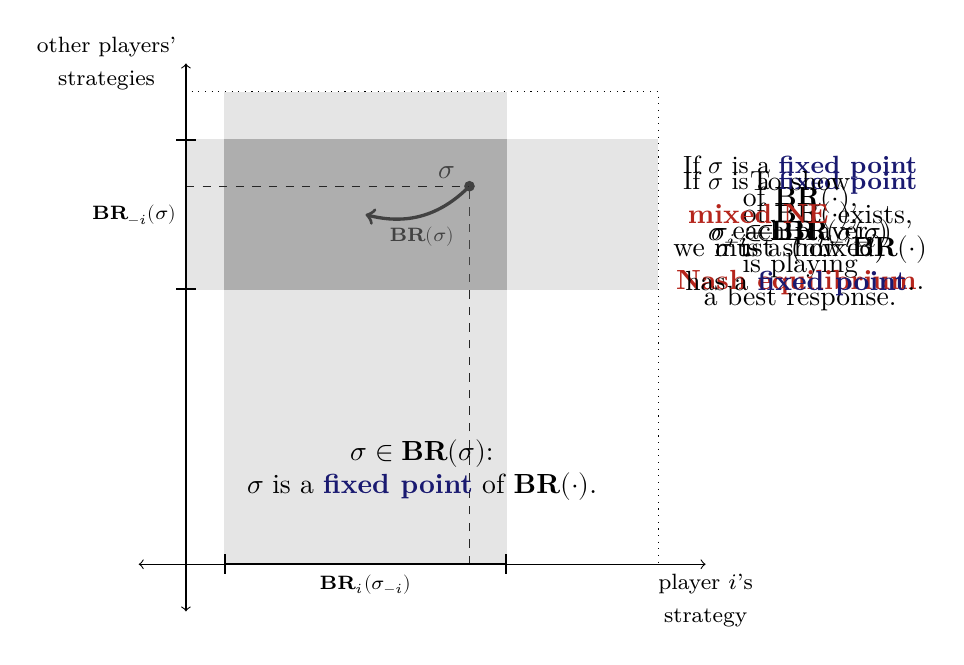
\begin{tikzpicture}[scale=1.2,domain=0:6]
    \coordinate (A) at (3.0,4.0);
    \coordinate (B) at (3.0,0);
    \coordinate (C) at (0,4.0);
    \coordinate (D) at (0.4,0);
    \coordinate (E) at (3.4,0);
    \coordinate (F) at (3.4,5);
    \coordinate (G) at (0.4,5);
    \coordinate (J) at (0,2.9);
    \coordinate (K) at (0,4.5);
    \coordinate (L) at (5,4.5);
    \coordinate (M) at (5,2.9);
    \coordinate (P) at (0.4,2.9);
    \coordinate (Q) at (3.4,2.9);
    \coordinate (R) at (3.4,4.5);
    \coordinate (S) at (0.4,4.5);
    \coordinate (T) at (1.9,3.7);
    \coordinate (U) at (2.5,1);
    \coordinate (V) at (6.5,3.5);
    \coordinate (W) at (6.5,2.5);
    \coordinate (X) at (6.5,1.5);
    \draw[dotted] (0,0) rectangle (5,5);
    %\draw[dotted,color=gray] (-0.1,-0.1) grid (5,5);
    \draw[<->] (-0.5,0) -- (5.5,0) node[below, align=center] {\footnotesize player $i$'s\\ \footnotesize strategy};
    \draw[<->] (0,-0.5) -- (0,5.3) node[left, align=center] {\footnotesize other players' \\ \footnotesize strategies};
    \draw[fill=black] (A) circle(0.05);
    \node[above=5,left=2] at (A) {$\sigma$};
    \fill[gray!200,nearly transparent] (P)--(Q)--(R)--(S) -- cycle;
    \path[->,very thick] (A) edge[bend left] node[below] {\scriptsize $\BR(\sigma)$} (T);
    \onslide<2>{
      \draw[dashed] (B) -- (A);
      \fill[gray!80,nearly transparent] (D)--(E)--(F)--(G) -- cycle;
      \draw[|-|, thick] (D) -- node[midway,below]{\scriptsize $\BR_i(\sigma_{-i})$} (E);      
      \node at (V) {$\sigma_i \in \BR_i(\sigma_{-i})$};
    }
    \onslide<3>{
      \draw[dashed] (C) -- (A);
      \fill[gray!80,nearly transparent] (J)--(K)--(L)--(M) -- cycle;
      \node at (V) {$\sigma_{-i} \in \BR_{-i}(\sigma)$};
      \draw[|-|, thick] (J) -- node[midway,left]{\scriptsize $\BR_{-i}(\sigma)$} (K);
    }
    \onslide<4->{\node[align=center] at (U) {$\sigma \in \BR(\sigma)$:\\ $\sigma$ is a \textbf{\textcolor{MidnightBlue}{fixed point}} of $\BR(\cdot)$.};}
    \onslide<5>{\node[align=center] at (V) {\small If $\sigma$ is a \textcolor{MidnightBlue}{\textbf{fixed point}}\\ of $\BR(\cdot)$,\\ each player\\ is playing\\ a best response.};}
    \onslide<6>{\node[align=center] at (V) {\small If $\sigma$ is a \textcolor{MidnightBlue}{\textbf{fixed point}}\\ of $\BR(\cdot)$,\\ $\sigma$ is a (mixed)\\ \textcolor{BrickRed}{\textbf{Nash equilibrium}}.};}
    \onslide<7>{\node[align=center] at (V) {To show \\\textcolor{BrickRed}{\textbf{mixed NE}} exists,\\ we must show $\BR(\cdot)$\\ has a \textcolor{MidnightBlue}{\textbf{fixed point}}.};}
\end{tikzpicture}
\end{frame}




\end{document}


%%% Local Variables:
%%% mode: latex
%%% TeX-master: t
%%% End:
